\documentclass[a4paper,12pt]{article}
\usepackage[german]{babel}
\usepackage[utf8]{inputenc}
\usepackage[margin=1in]{geometry}
\usepackage{amsmath}
\usepackage{graphicx}

\setlength\parindent{0pt}

\begin{titlepage}

\begin{document}

\begin{center}
\large
Software Engineering\\
Studiengang Angewandte Informatik - Technische Hochschule Deggendorf\\
Wintersemester 16/17

\begin{center}
\Large
\vspace*{3\baselineskip}
\textbf{Dokumentation - Projekt Bordcomputer}
\vspace*{3\baselineskip}
\noindent\rule{16cm}{0.4pt}
\end{center}

\textbf{Globosoft AG}\\

Alexander Kainz, Florian Graßl, Matthias Baumgartner, Nicolas Tiefnig\\

\today

\end{center}

\end{titlepage}

\tableofcontents

\section{Zusammenfassung}

Bei dem Projekt Bordcomputer soll ein lauffähiges Programm entstehen, das als Bordcomputer im Automotive Bereich eingesetzt werden kann. Zusätzlich wird ein Simulator implementiert der ein Motorsteuergerät simulieren soll, das Werte an den Bordcomputer liefert und auch als Schnittstelle des Testers zu dem System dient. Insgesamt besteht die Software also aus dem Simulator und der eigentlichen Bordcomputer Software. Es wird zuerst eine Analyse der Requirements des Auftraggebers durchgeführt, um alle Anforderungen erfüllen zu können. Danach erfolgt Entwurf, Konzeption und Codierung mit einer abschließenden Testphase. Alle Arbeitsschritte werden in diesem Dokument zusammengefasst und detailliert erläutert.

\section{Anforderungsanalyse}

\subsection{Lastenheft}

Seitens des Auftraggebers liegen folgende Anforderungen an die Software in Form eines Lastenhefts vor (Original):\\

\noindent\rule{16cm}{0.4pt}
Lastenheft\\

Allgemeines:
Der Bordcomputer soll dem Fahrer Informationen über den aktuellen Fahrzeugzustand mitteilen. Im Einzelnen sind dies folgende Daten:

\begin{itemize}

\item Aktuelle Geschwindigkeit 
\item Temperatur Motoröl
\item Temperatur Kühlwasser
\item Außentemperatur 
\item Kraftstoffverbrauch momentan 
\item Kraftstoffverbrauch seit Fahrantritt
\item Seit Fahrtantritt zurückgelegte Strecke in km
\item Seit Fahrtantritt vergangene Zeit
\item Seit Fahrtantritt erreichte Durchschnittsgeschwindigkeit 
\item Warnung bei Erreichen einer eingestellten Maximalgeschwindigkeit

\end{itemize}
 
Die Software soll in einer PC Umgebung entwickelt und simuliert werden.

Anforderungen im Detail:

\begin{itemize}

\item Der Bordcomputer ist im Fahrbetrieb immer aktiv 
\item Über einen Schalter im Blinkhebel kann zwischen den Daten hin und her gewechselt werden 
user input / entscheidet über angezeigte Daten
\item Über einen zweiten Taster im Blinkhebel können die Daten, die seit Fahrtantritt gesammelt wurden, zurückgesetzt werden.
\item Mittels beider Taster soll eine Maximalgeschwindigkeit einstellbar sein, bei deren Erreichen eine Warnung ausgegeben wird. Die Warnung bleibt so lange erhalten, bis die eingestellte Maximalgeschwindigkeit wieder eingehalten wird.
\item Die angezeigten Daten werden aus den vom Fahrzeug über einen Kommunikations­bus gelieferten Daten (aktuelle Geschwindigkeit, aktueller Verbrauch, Öl- und Wassertemperatur, Außentemperatur) berechnet. 
\item Die Anzeige des Bordcomputers darf grafisch oder alphanumerisch implementiert werden.
\item Zum Test des Bordcomputers ist zusätzlich eine Simulationssoftware zu erstellen, die dem Bordcomputer die vom Fahrzeug gelieferten und benötigten Daten (aktueller Verbrauch, aktuelle Geschwindigkeit, Temperaturen von Motoröl und Kühlwasser, Zündung an/aus usw.) und die Tasterstellung permanent zur Verfügung stellt.

\end{itemize}
\noindent\rule{16cm}{0.4pt}

\subsection{Überarbeitung Lastenheft}

An dem Lastenheft werden seitens des Projektteams folgende Ergänzungen vorgenommen:\\

Lastenheft (von Projektteam überarbeitet)

\begin{itemize}

\item Aktuelle Geschwindigkeit

		\textbf{Annahme:} \emph{Aktuelle Geschwindigkeit wird jede Sekunde vom Simulator geliefert}

\item \textbf{Temperatur} Motoröl 
\item \textbf{Temperatur} Kühlwasser
\item Außen\textbf{temperatur}

		\textbf{Ergänzung:} \emph{Alle Temperaturen werden von Simulator vorgegeben}

\item Kraftstoffverbrauch momentan

		\textbf{Annahme:} \emph{Kraftstoffverbrauch wird von Simulator vorgegeben (Drosselklappenstellung) und jede Sekunde vom Simulator geliefert}

\item Kraftstoffverbrauch \textbf{Seit Fahrtantritt}
\item \textbf{Seit Fahrtantritt} zurückgelegte Strecke in km
\item \textbf{Seit Fahrtantritt} vergangene Zeit
\item \textbf{Seit Fahrtantritt} erreichte Durchschnittsgeschwindigkeit

		\textbf{Ergänzung:} \emph{Anforderung: Zeit seit Fahrantritt muss zuverlässig gezählt werden}

\item \textbf{Warnung} bei Erreichen einer eingestellten Maximalgeschwindigkeit

		\textbf{Ergänzung:} \emph{Warnung definiert als Ausrufezeichen in der alphanumerischen Anzeige}
		
Die Software soll in einer PC Umgebung entwickelt und simuliert werden.

\textbf{Ergänzung:} \emph{Gesamte Software soll auf einem Windows 7 (32/64-Bit) Betriebssystem lauffähig sein}

%\begin{itemize}

\item Der Bordcomputer ist im Fahrbetrieb immer aktiv

\textbf{Annahme:} \emph{Fahrbetrieb beginnt wenn Zündung erfolgt}

\item Über einen \emph{Schalter} im Blinkhebel kann zwischen den Daten hin und her gewechselt werden 
user input / entscheidet über angezeigte Daten

\textbf{Anmerkung:} \emph{Hier wird von einem Schalter gesprochen, gemeint wird aber ein Taster}

\item Über einen zweiten Taster im Blinkhebel können die Daten, die seit Fahrtantritt gesammelt wurden, zurückgesetzt werden. 

\textbf{Annahme:} \emph{Die beiden Taster und deren Stellung wird vom Simulator vorgegeben.}

\textbf{Annahme:} \emph{Es werden alle Daten gemeint (Verbrauch, Strecke, Durchschnittsgeschwindigkeit usw.), ab dem Zeitpunkt des Reset erfolgt eine neue Messung der Daten.}

\item Mittels beider Taster soll eine Maximalgeschwindigkeit einstellbar sein, bei deren Erreichen eine Warnung ausgegeben wird. Die Warnung bleibt so lange erhalten, bis die eingestellte Maximalgeschwindigkeit wieder eingehalten wird.

\textbf{Anmerkung:} \emph{Maximalgeschwindigkeit wird vom Simulator als positive Ganzzahl vorgegeben}

\item Die angezeigten Daten werden aus den vom Fahrzeug über einen Kommunikations­bus gelieferten Daten (aktuelle Geschwindigkeit, aktueller Verbrauch, Öl- und Wassertemperatur, Außentemperatur) berechnet. 

\textbf{Anmerkung:} \emph{Der Kommunikationsbus wird vom Simulator "ersetzt", Werte werden durch den Simulator eingestellt und an die Bordcomputer Software geschickt}

\item Die Anzeige des Bordcomputers darf grafisch oder alphanumerisch implementiert werden.

\textbf{Anmerkung:} \emph{Da sich die Anzeige eines Automobils nur schwer auf einem Computer nachbilden lässt (LCD-Display) wird auf ein GUI verzichtet}

\item Zum Test des Bordcomputers ist zusätzlich eine Simulationssoftware zu erstellen, die dem Bordcomputer die vom Fahrzeug gelieferten und benötigten Daten (aktueller Verbrauch, aktuelle Geschwindigkeit, Temperaturen von Motoröl und Kühlwasser, Zündung an/aus usw.) und die Tasterstellung permanent zur Verfügung stellt.

\textbf{Ergänzung:} \emph{Einheitenfestlegung:}

*Temperaturen Anzeige in Grad $C^{\circ}$\\
*Kraftstoffverbrauch Anzeige in $Liter/100 Kilometer$\\
*Geschwindigkeiten Anzeige in $Kilometer/Stunde$

\textbf{Anmerkung:} \emph{Die Software besteht aus zwei Teilen. Zum einen aus der Bordcomputersoftware selbst und einem Simulator}

\end{itemize}

Um eine einfache, übersichtliche Darstellung des Lastenhefts zu erzielen, wird ein Diagram angefertigt, dass alle Anforderungen grafisch darstellt.

\begin{figure}[ht]

\begin{center}
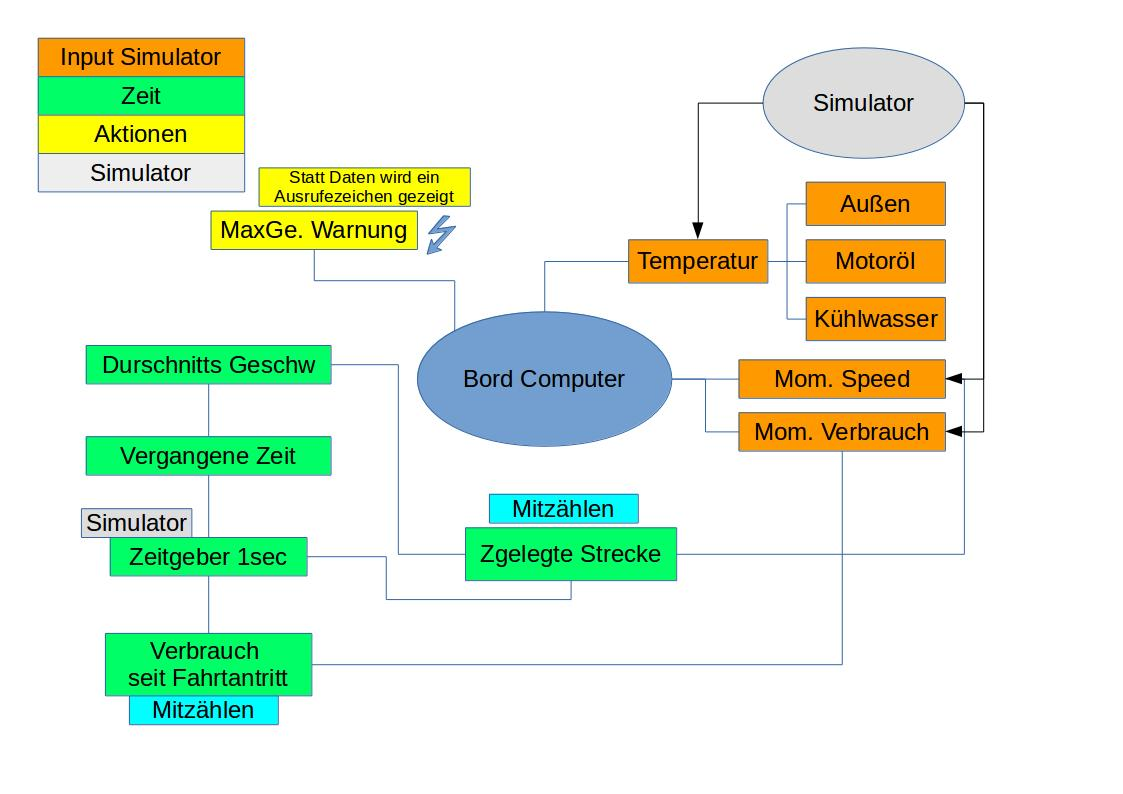
\includegraphics[scale=0.55]{Requirements_v2.jpg}
\caption{Grafische Darstellung der Anforderung}
\end{center}

\end{figure}

Nun liegen die Anforderungen an die Software detailliert und nachvollziehbar vor, das Diagram dient als Rahmen für die nächsten Schritte der Entwicklung.

\subsection{Unterteilung des Systems in Funktionsgruppen}

Das Gesamtsystem wird der Übersicht halber in einzelne Funktionseinheiten unterteilt, die Unterteilung liegt ebenfalls in Form eines Diagrams vor (Abbildung 2, Seite 6).

\begin{figure}[!ht]

\begin{center}
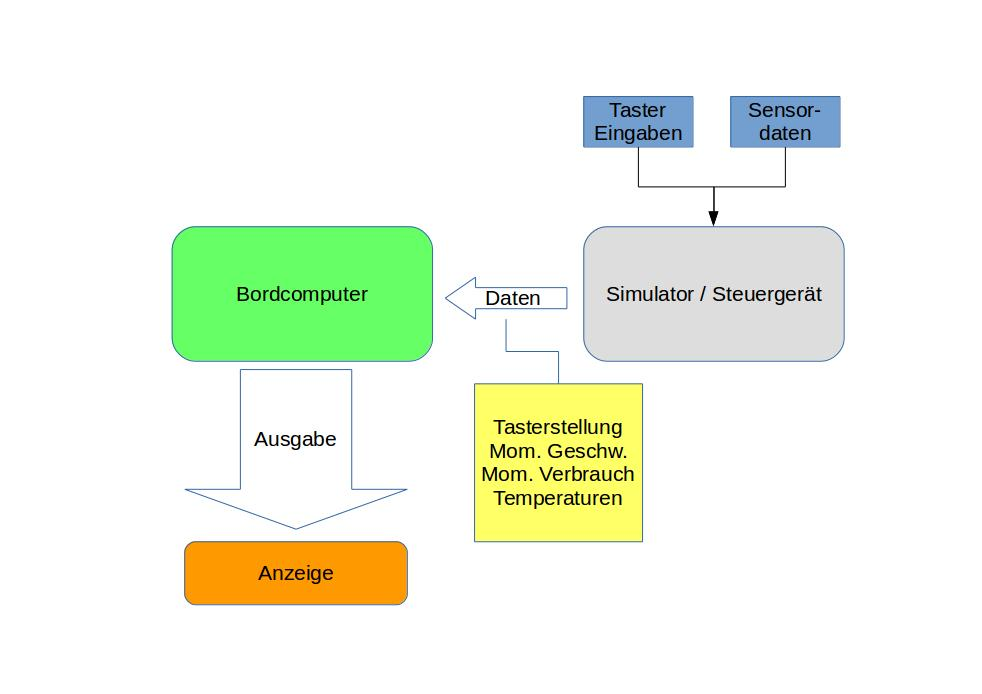
\includegraphics[scale=0.55]{Funktionsblock.jpg}
\caption{Einteilung in Funktionsgruppen}
\end{center}

\end{figure}

\subsubsection{Bordcomputer}

Die Anzeigewerte des Bordcomputers werden in folgender Reihenfolge dargestellt:
\begin{enumerate}
	\item Momentangeschwindigkeit
	\item Durchschnittsgeschwindigkeit
	\item Momentanverbrauch
	\item Durchschnittsverbrauch
	\item Gefahrene Strecke seit Fahrtantritt
	\item Vergangene Zeit seit Fahrtantritt
	\item Maximalgeschwindigkeit
\end{enumerate}

Nähere Definition der Anzeigewerte:
\begin{enumerate}
	\item Momentangeschwindigkeit 
			wird in km/h angezeigt
	\item Durchschnittsgeschwindigkeit
			wird in km/h angezeigt
	\item Momentanverbrauch
			wird in l/100km angezeigt wenn das Fahrzeug in Bewegung ist,
			Steht das Fahrzeug still wird ein Bindestrich angezeigt
	\item Durchschnittsverbrauch
			wird in l/100km angezeigt
	\item Gefahrene Strecke seit Fahrtantritt
			wird in km angezeigt
	\item Vergangene Zeit seit Fahrtantritt
			wird in Stunden und Minuten angezeigt
	\item Maximalgeschwindigkeit
			wird in km/h angezeigt
\end{enumerate}

Allgemeine Festlegungen:

\begin{itemize}

	\item alle Verbrauchswerte werden mit zwei Nachkommastellen angezeigt
	\item alle Geschwindigkeiten ohne Nachkommastellen
	\item alle Strecken mit einer Nachkommastelle

\end{itemize}

\subsubsection{Simulator}

Eigenschaften und Festlegungen der Tastereingaben:\\

Taster 1
\begin{itemize}

	\item wechselt zwischen den Daten die von der Anzeige dargestellt werden
	\item Bei der Auswahl der Maximalgeschwindigkeit ist dieser Taster derjenige, der den einzustellenden Wert erhöht

\end{itemize}

Taster 2
\begin{itemize}

	\item Rücksetzen aller Werte seit Fahrtantritt (Durchschnittsverbrauch, Durchschnittsgeschwindigkeit und Strecke) auf null
	\item Bei der Auswahl der Maximalgeschwindigkeit ist dieser Taster derjenige, der den einzustellenden Wert erniedrigt
	
\end{itemize}

Taster 1 und Taster 2 in Kombination
\begin{itemize}

	\item Aufruf Menü zur Einstellung der Maximalgeschwindigkeit.
	\item Taster 1 Maximalgeschw. +10 km/h, Taster 2 Maximalgeschw. -10 km/h.
	\item Nochmaliges Drücken beider Taster speichert der Maximalgeschw. Rückkehr zum vorherigen Menüpunkt.
	\item negative Werte sind nicht einstellbar, eine Null wird als Bindestrich dargestellt und bedeutet dass keine Maxmimalgeschwindigkeit eingestellt ist
	\item Null ist der Ausgangswert nach Einschalten der Zündung
	\item Werden beide Taster erneut betätigt um das Menü zur Einstellung der Maximalgeschwindigkeit aufzurufen wird der zuletzt eingestellte Wert angezeigt
	
\end{itemize}

Die Werte der Taster werden intern als Wahrheitswerte dargestellt und übergeben (true/false).

\subsection{Spezifikationen der Funktionsgruppen}



\end{document}